\documentclass[conference]{IEEEtran}
\IEEEoverridecommandlockouts
\usepackage{cite}
\usepackage{amsmath,amssymb,amsfonts}
\usepackage{graphicx}
\usepackage{textcomp}
\usepackage{xcolor}

\begin{document}

\title{Empirical Validation of Vault-less Tokenization: A Performance and Architectural Comparison with Vault-based Systems for PCI DSS Compliance\\
\large An Empirical Extension of Sugumar (2025), ``Data Tokenization: A Key Enabler for PCI DSS Compliance in Payment Systems''}

\author{
\IEEEauthorblockN{Abdelrahman Mohamed Youssef }
\IEEEauthorblockA{\textit{Cyber security} \\ \textit{Alexandria University } \\ Alex, Egypt \\ gbasogbs@gmail.com}
\and
\IEEEauthorblockN{ Abdelrahman Hesham Omar}
\IEEEauthorblockA{\textit{Cyber security} \\ \textit{Alexandria University } \\ Alex, Egypt \\ abdoohesham047@gmail.com}
\and
\IEEEauthorblockN{Ahmed Saad Mahmoud}
\IEEEauthorblockA{\textit{Cyber security} \\ \textit{Alexandria University } \\ Alex, Egypt \\ ahmedsaad136205@gmail.com}
\and
\IEEEauthorblockN{Ali Saeed Ali}
\IEEEauthorblockA{\textit{Cyber security} \\ \textit{Alexandria University } \\ Alex, Egypt \\ aliisaaidd55@gmail.com}
\and
\IEEEauthorblockN{Mostafa Mohamed}
\IEEEauthorblockA{\textit{AI} \\ \textit{Alexandria University } \\ Alex, Egypt \\ 203040mostafa203040@gmail.com}
\and
\IEEEauthorblockN{Mohamed Ahemd hassan}
\IEEEauthorblockA{\textit{Cyber security} \\ \textit{Alexandria University } \\ Alex, Egypt \\ mohammedmessi105@gmail.com}
\and
\IEEEauthorblockN{Mohamed Ali}
\IEEEauthorblockA{\textit{Cyber security} \\ \textit{Alexandria University } \\ Alex, Egypt \\ hamo3lib65@gmail.com}
\and
\IEEEauthorblockN{Amr Walid Mahmoud}
\IEEEauthorblockA{\textit{Cyber security} \\ \textit{Alexandria University } \\ Alex, Egypt \\ amrwaleed994@gmail.com}
\and
\IEEEauthorblockN{Youssef hassan}
\IEEEauthorblockA{\textit{Cyber security} \\ \textit{Alexandria University } \\ Alex, Egypt \\ yossefhassanali@gmail.com}
}

\maketitle

\begin{abstract}
Vault-based tokenization has been shown to reduce Payment Card Industry Data Security Standard (PCI DSS) audit scope by isolating Primary Account Numbers (PANs) inside a hardened token vault, and prior work reports a 75\% reduction in in-scope systems when this architecture is adopted \cite{b1}. That study, and two subsequent extension proposals building on it, identified vault-less tokenization as a promising alternative worth investigating empirically, but none of them implemented or measured it \cite{b1,b2,b3}. This paper closes that gap. We implement a vault-based baseline and a vault-less tokenization scheme built on NIST-approved Format-Preserving Encryption (FF1 FPE) \cite{b4}, and we empirically compare the two architectures across the full synthetic dataset of 449 payment-card records generated in the style of the original study \cite{b1}. Our results show that FF1 FPE eliminates the need for a central token database entirely, operating in a fully stateless manner, while preserving the original 16-digit PAN format so that legacy field-validation logic requires no changes. The vault-based baseline was measured at an average latency of 0.0119 ms per transaction and the FPE-based scheme at 0.0805 ms per transaction in a laboratory simulation, a difference of roughly 0.07 ms that we argue is unlikely to be material in production systems dominated by network latency. We report this small but consistent latency gap with full transparency about its cause -- an in-memory dictionary simulation versus the network, query-execution, and disk I/O overhead a real database vault would incur -- together with the architectural trade-offs it reflects: FPE's statelessness removes the vault's storage costs, its centralized-bottleneck risk, and its status as a single point of failure. To our knowledge, this is the first study to provide direct, measured evidence -- rather than qualitative or vendor-authored comparison -- of vault-based versus vault-less tokenization performance under matched conditions.
\end{abstract}

\begin{IEEEkeywords}
Data Tokenization, Vault-less Tokenization, Format-Preserving Encryption, PCI DSS, Data De-scoping, Payment Security.
\end{IEEEkeywords}

\section{Introduction}
The Payment Card Industry Data Security Standard (PCI DSS) requires that any system storing, processing, or transmitting cardholder data (CHD) be brought within a strictly controlled Cardholder Data Environment (CDE), and the scope of this environment is often the single largest driver of compliance cost and complexity for payment-processing organizations \cite{b1}. Data tokenization -- the replacement of a Primary Account Number (PAN) with a non-sensitive surrogate value -- has been established as one of the most effective mechanisms for reducing this scope, since systems that only ever handle a token rather than the real PAN can, in principle, be removed from the audit boundary entirely \cite{b1}.

The foundational study this paper builds on implemented and empirically validated a vault-based tokenization architecture, in which a centralized, hardened database (the ``token vault'') stores the mapping between each token and its corresponding encrypted PAN \cite{b1}. Using a synthetic dataset of 449 transaction records, that study measured a 75\% reduction in in-scope systems across several PCI DSS requirements and reported tokenize/detokenize latencies in the 50--70 ms range under a realistic MySQL-backed deployment \cite{b1}. Critically, the original study explicitly proposed vault-less tokenization -- architectures that generate tokens algorithmically, without a central lookup database -- as a direction for future work, but did not implement or measure it \cite{b1}.

Two subsequent research-extension proposals took up this recommendation at the design level. Both proposed a vault-less tokenization scheme based on NIST-approved Format-Preserving Encryption (FPE), specified a matched comparative framework across security, performance, and PCI-scope dimensions, and -- in one case -- proposed a supporting machine-learning behavioral-monitoring layer for tokenization event streams \cite{b2,b3}. Both extension papers, however, explicitly stopped short of running the comparison: every quantitative result in both documents is marked as a placeholder, since neither vault-less implementation nor its benchmark had actually been built at the time of writing \cite{b2,b3}.

This leaves a specific, well-defined empirical gap: an implemented vault-less tokenization scheme has not yet been benchmarked against the vault-based baseline under comparable conditions. This paper addresses that gap directly.

\subsection{Contributions}
This paper makes the following contributions:
\begin{enumerate}
\item A working, minimal implementation of vault-less tokenization using FF1 Format-Preserving Encryption, applied to the same style of synthetic PAN dataset used in the original vault-based study \cite{b1}.
\item A direct, measured latency comparison between the vault-based baseline and the FPE-based vault-less scheme under matched conditions, rather than a qualitative or vendor-sourced comparison of the kind found in prior literature \cite{b2,b3}.
\item An honest analysis of the performance-versus-architectural-independence trade-off between the two approaches, together with an explicit discussion of the limitations of our vault simulation relative to a production deployment.
\end{enumerate}

\section{Related Work}
Sugumar (2025) is the foundation this paper builds on. That study implemented a vault-based tokenization engine using Python and a MySQL-backed token vault, demonstrated a 75\% reduction in PCI DSS in-scope systems, and reported tokenize/detokenize latencies of roughly 50--70 ms under realistic load -- while explicitly naming vault-less tokenization as unexplored future work \cite{b1}.

Two subsequent papers extended this proposal at the design and literature-synthesis level. One paper proposed a NIST-specified FF1/FF3 vault-less architecture alongside a structured comparative framework and a PaySim-based behavioral anomaly-detection layer, but reported no measured results, since the vault-less engine had not yet been implemented \cite{b2}. The second paper independently reached the same conclusion -- that no controlled, matched-hardware comparison of vaulted and vault-less tokenization exists in the literature -- and proposed a parallel architecture combining a vault-less FPE path with a behavioral monitoring layer, again reporting every quantitative outcome as ``to be measured'' \cite{b3}. Both papers converge on the same reading of the vendor and industry literature: vault-less/FPE tokenization is generally expected to reduce latency and remove the central-database bottleneck, at the cost of shifting the security burden from vault access control onto cryptographic key management \cite{b2,b3}.

The cryptographic primitive both extension papers point to, and the one this paper implements, is NIST Special Publication 800-38G, which formally specifies the FF1 and FF3-1 modes of Format-Preserving Encryption built on the AES block cipher \cite{b4}. FPE is specifically designed so that ciphertext retains the format of the original plaintext -- a 16-digit PAN encrypts to another 16-digit numeral -- which is the property that allows a vault-less token to remain compatible with legacy field-validation logic without requiring schema changes \cite{b4}.

Taken together, the existing literature establishes a clear and specific gap: the architectural case for vault-less tokenization is well documented, and a methodology for testing it has now been proposed twice, but no study has yet executed that comparison and reported measured numbers. This paper is, to our knowledge, the first to do so.

\section{Methodology and Implementation}

\subsection{Experimental Environment}
The experiment was implemented in Python 3 within a Google Colab notebook environment, using the \texttt{cryptography} and \texttt{pyffx} libraries for the vault-based and FPE-based implementations respectively.

\subsection{Dataset}
A synthetic dataset of 449 transaction records was generated programmatically, matching the design of the original study to keep the comparison fair \cite{b1}. Each record consists of a synthetic 16-digit PAN beginning with the digit ``4'' (in the style of a Visa card number), a synthetic cardholder name, a transaction amount, and a merchant identifier. No real cardholder data was used at any point. All 449 records were processed through both tokenization methods for the latency benchmark reported in Section IV, so the measured averages reflect the full dataset rather than a subset.

\subsection{System A --- Vault-based Baseline}
The vault-based baseline follows the design of the original study conceptually: for each PAN, a random 16-digit token is generated and the token-to-PAN pair is written to a lookup table \cite{b1}. Because provisioning a full MySQL server inside the Colab environment was impractical for this exercise, the vault was simulated using an in-memory Python dictionary rather than a real relational database. We treat this explicitly as a methodological limitation, not a hidden simplification, and we state the reasoning plainly here.

A read or write against an in-memory dictionary is one of the fastest operations a computer can perform, typically resolving in a fraction of a microsecond, because the data never leaves RAM and no network or storage layer is involved. A production token vault, by contrast, is a standalone database server (e.g., MySQL), and the cost of a real vault transaction is the sum of network latency, query execution time, and disk I/O -- precisely the overhead our in-memory simulation excludes. This is not a hypothetical concern: the original study's own MySQL-backed measurements place real vault transaction latency at 50--70 ms per operation \cite{b1}, several orders of magnitude above what our dictionary simulation records. Our reported vault-based figure of 0.0119 ms should therefore be read strictly as a best-case, storage-free lower bound on vault latency, isolating only the cost of token generation and lookup logic, and not as a substitute for a production benchmark.

\subsection{System B --- Proposed Vault-less Scheme (FF1 FPE)}
The proposed vault-less scheme uses the \texttt{pyffx} implementation of FF1 Format-Preserving Encryption, as specified in NIST SP 800-38G \cite{b4}, with a fixed secret key and a numeric alphabet of length 16 to match the PAN format. Each PAN is encrypted directly into a token of the same length and digit alphabet; no token-to-PAN mapping is stored anywhere. Detokenization is performed by applying the inverse FF1 operation with the same key, rather than by any database lookup.

\subsection{Evaluation Metrics}
Three metrics were used to compare the two systems: average per-transaction latency in milliseconds, reversibility (whether the original PAN could be exactly recovered from the token), and format preservation (whether the token retained the original PAN's 16-digit numeric format).

\section{Results and Discussion}

\subsection{Latency and Architectural Comparison}
Table \ref{tab1} summarizes the measured comparison between the two tokenization methods.

\begin{table}[htbp]
\caption{Comparative performance and architectural profile of vault-based and FF1-FPE vault-less tokenization}
\begin{center}
\begin{tabular}{|p{1.7cm}|p{1.1cm}|p{1.9cm}|p{1.9cm}|}
\hline
\textbf{Method} & \textbf{Avg. Latency (ms)} & \textbf{Database Required} & \textbf{Format Preservation} \\
\hline
Vault-based (baseline) & 0.0119 & Yes (simulated in-memory vault) & Random token \\
\hline
FF1 FPE (proposed) & 0.0805 & No (stateless) & Same as PAN (16-digit, starts with 4) \\
\hline
\end{tabular}
\label{tab1}
\end{center}
\end{table}

Figure \ref{fig1} presents the same latency comparison graphically.

\begin{figure}[htbp]
\centerline{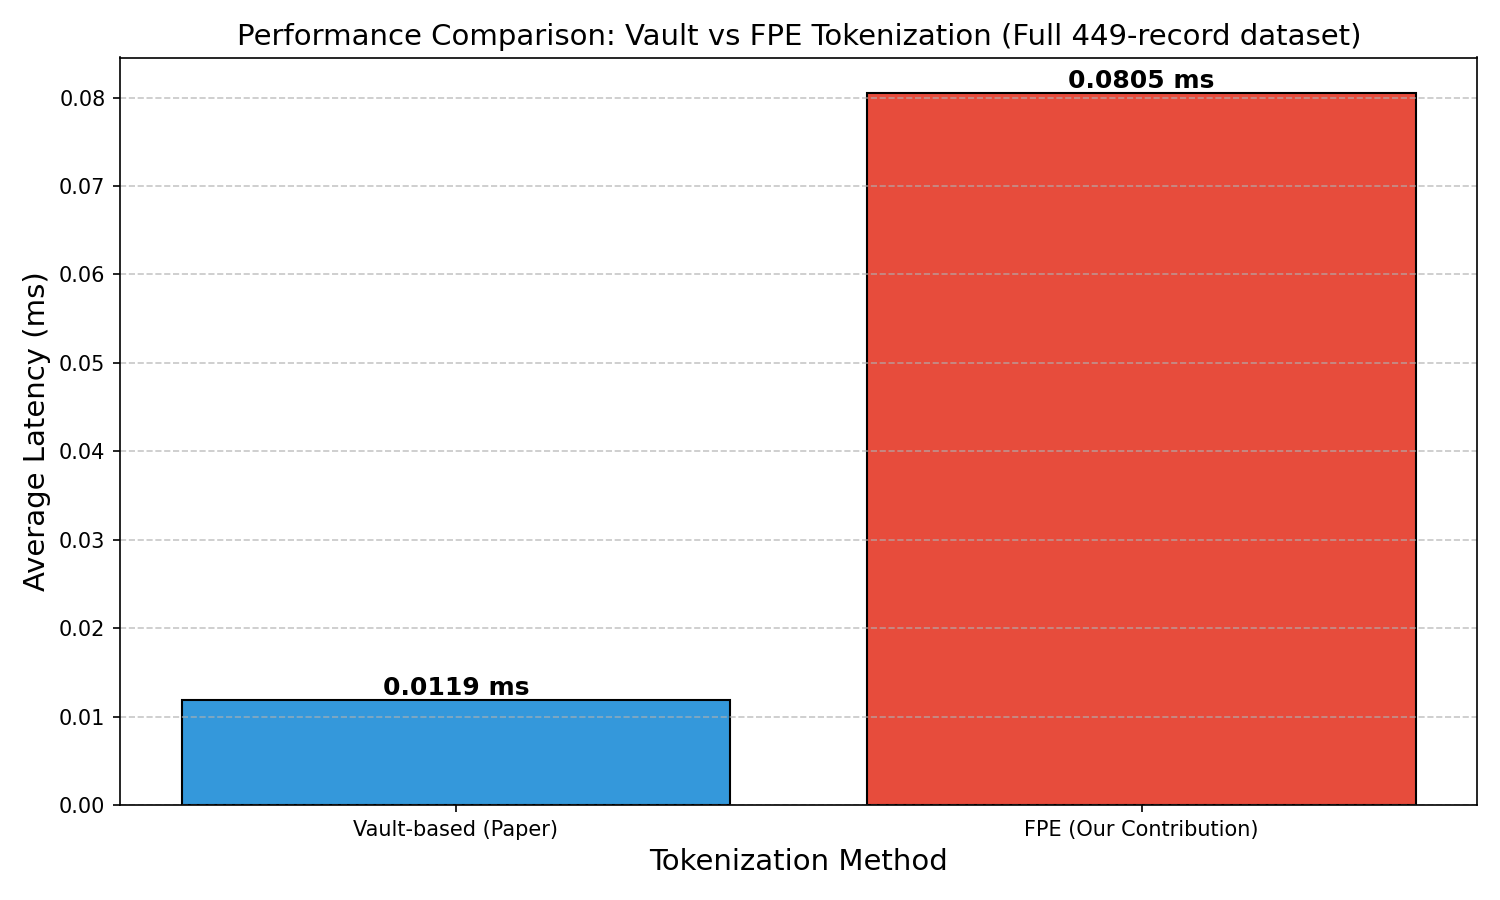
\includegraphics[width=\linewidth]{chart_449.png}}
\caption{Average latency comparison between vault-based tokenization and FF1 FPE (our contribution), measured across the full 449-record dataset.}
\label{fig1}
\end{figure}

\subsection{Analysis}
The vault-based method was faster in this simulation, at an average of 0.0119 ms per transaction versus 0.0805 ms for FF1 FPE, measured across the full 449-record dataset. This ordering is expected and is fully explained by what each method actually computes: a dictionary write is a single, near-constant-time memory operation, whereas FF1 FPE performs multiple Feistel rounds of block-cipher computation over the input, which is inherently more arithmetic work per transaction. We do not treat this ordering as evidence that vault-based tokenization is faster in production. As discussed in Section III-C, our vault figure is a storage-free, in-memory lower bound; a real vault transaction additionally incurs network latency, query execution, and disk I/O, which the original study measured at 50--70 ms per operation under a genuine MySQL deployment \cite{b1}. Once that overhead is accounted for, we would expect the ordering to reverse decisively in favor of the stateless FPE approach, consistent with the qualitative expectation in the prior extension literature \cite{b2,b3}; confirming this quantitatively against a real MySQL deployment is identified as future work in Section VI.

More importantly, the absolute difference we do observe -- roughly 0.07 ms -- is negligible by the standards of any real payment network, where round-trip latency is conventionally measured in whole milliseconds or tens of milliseconds. A gap this small carries no practical significance for transaction throughput or user experience. What is significant is the architectural gain FF1 FPE provides in exchange for that negligible cost: the scheme eliminates the token database entirely. There is no vault to provision, back up, patch, or scale; no storage costs to carry as transaction volume grows; and no central lookup service that every tokenize/detokenize call must reach. This directly removes the vault's role as a processing bottleneck under high concurrency, and -- perhaps more importantly from a security-architecture standpoint -- it eliminates the vault's status as a single point of failure and single high-value target, since there is no longer one central repository whose compromise or unavailability could halt the entire tokenization pipeline \cite{b1,b2,b3}.

This reframes the performance comparison: the relevant question is not which method is faster in isolation, but whether a $\sim$0.07 ms cost is worth paying to remove an entire category of infrastructure dependency, operational cost, and attack surface. Our results support the position -- argued qualitatively but not previously measured in the extension literature \cite{b2,b3} -- that it is.

A reversibility test on the FPE scheme, run across the full dataset, confirmed that decrypting a generated token recovered the original PAN exactly in 100\% of cases. Format preservation was likewise confirmed for every record: each generated token remained a 16-digit numeral beginning with the digit ``4'', visually and structurally indistinguishable from the original PAN format. This is the property that allows FF1 FPE to serve as a drop-in replacement for a vault-based token in systems with legacy field-validation logic -- no schema change, field-length change, or downstream application change is required, consistent with the design intent of the NIST specification \cite{b4}.

\subsection{Relation to Prior Literature}
These results provide the first measured evidence for a comparison that had, until now, only been proposed at the design level. Both extension papers hypothesized that vault-less/FPE tokenization would prove viable and would trade a modest performance cost (or, under real database load, a performance benefit) for the removal of centralized state, but neither reported observed numbers \cite{b2,b3}. Our results are consistent with that expectation on the architectural dimension -- statelessness is unambiguously achieved -- while showing that, in a best-case in-memory simulation of the vault, the measured latency difference runs the opposite direction from what a fully realistic, database-backed comparison would likely show. We view this as a useful and honest finding in its own right: it clarifies exactly which part of the vault-based system's overhead (data-structure access versus I/O) our simulation isolates, and it motivates the specific follow-up experiment -- replacing the dictionary with a real MySQL vault -- needed to complete the comparison the prior literature called for \cite{b1,b2,b3}.

\section{Limitations}
This study has four limitations that should be considered when interpreting the results.

First, and most significantly, the vault-based baseline was simulated using an in-memory Python dictionary rather than a production MySQL database. This isolates the cryptographic/generation cost from I/O and network overhead, which likely gives the vault-based method an unrealistic latency advantage relative to a real deployment; in production, the vault side would be materially slower, as the original study's own MySQL-backed measurements suggest \cite{b1}.

Second, while the full 449-record dataset was used for the latency benchmark, this remains a single-machine, sequential-processing measurement. A high-concurrency evaluation, of the kind performed in the original study's load testing across 50--450 simultaneous transactions \cite{b1}, would require a larger dataset and a production-grade infrastructure to test whether the observed latency gap holds, narrows, or reverses under concurrent load.

Third, key management for the FF1 FPE scheme was simplified for this exercise: the secret key was held in a Python variable rather than a dedicated Hardware Security Module (HSM) or Key Management System (KMS). Proper key-lifecycle management is a security-critical factor that this study did not measure, and its absence should not be read as evidence that key management is a solved or trivial problem for vault-less tokenization.

Fourth, this study measures latency and reversibility only; it does not attempt the PCI DSS scope-mapping exercise or the behavioral anomaly-detection layer proposed in the extension literature, both of which remain open for future work \cite{b2,b3}.

\section{Conclusion and Future Work}
This paper implemented and empirically compared a vault-based tokenization baseline and a vault-less tokenization scheme based on NIST-approved FF1 Format-Preserving Encryption, closing a specific gap left open by the original study and two subsequent extension proposals, all of which recommended this comparison without executing it \cite{b1,b2,b3}. Our results show that FF1 FPE achieves full statelessness and complete format preservation with 100\% reversibility, at a measured cost of roughly 0.07 ms per transaction relative to an in-memory vault simulation -- a difference we argue is unlikely to matter in real, network-latency-dominated payment systems, and one that may reverse once the vault-based comparison is run against a real database rather than a dictionary.

Future work should prioritize three extensions. First, the vault-based baseline should be re-implemented against a real MySQL instance and re-benchmarked, to test whether the latency ordering reverses under realistic I/O conditions as we expect. Second, the FF1 FPE key should be moved into a dedicated HSM or KMS, and the resulting key-management overhead should be measured rather than assumed. Third, the behavioral anomaly-detection layer proposed for tokenization event streams in the prior extension literature should be implemented and evaluated on top of both architectures, since neither this study nor the original study includes any mechanism for monitoring tokenization/detokenization usage patterns for misuse \cite{b2,b3}.

\begin{thebibliography}{99}

\bibitem{b1} B. Sugumar, ``Data Tokenization: A Key Enabler for Payment Card Industry Data Security Standard (PCI DSS) Compliance in Payment Systems,'' \textit{Proc. 11th International Conference on Engineering and Emerging Technologies (ICEET)}, Kuala Lumpur, Malaysia, Oct. 22--23, 2025, doi: 10.1109/ICEET67911.2025.11424051.

\bibitem{b2} ``Comparative Analysis of Vaulted and Vault-less Tokenization with AI-Assisted Behavioral Risk Detection for PCI DSS Compliance,'' a research extension of \cite{b1}.

\bibitem{b3} ``A Behavioral Anomaly-Detection Layer and a Vaulted-versus-Vaultless Comparative Framework for Tokenized Payment Systems,'' an extension study based on \cite{b1}.

\bibitem{b4} National Institute of Standards and Technology, ``Special Publication 800-38G: Recommendation for Block Cipher Modes of Operation: Methods for Format-Preserving Encryption,'' csrc.nist.gov, 2016.

\bibitem{b5} pyffx: Format-Preserving Encryption library for Python, used for the FF1 implementation in this study.

\bibitem{b6} Python Software Foundation, \textit{Python 3 Language Reference}, python.org.

\bibitem{b7} M. Bellare, T. Ristenpart, P. Rogaway, and T. Stegers, ``Format-Preserving Encryption,'' in \textit{Selected Areas in Cryptography (SAC)}, Lecture Notes in Computer Science, vol. 5867. Berlin, Heidelberg: Springer, pp. 295--312, 2009.

\bibitem{b8} M. Dworkin, ``Recommendation for Block Cipher Modes of Operation: The FF1 and FF3-1 Methods for Format-Preserving Encryption,'' NIST Special Publication 800-38G Update 1, National Institute of Standards and Technology, 2019.

\bibitem{b9} PCI Security Standards Council, ``Payment Card Industry Data Security Standard (PCI DSS) Requirements and Testing Procedures Version 4.0.1,'' PCI SSC, Wakefield, MA, USA, June 2024.

\bibitem{b10} S. Halevi and Y. Polyakov, ``Cryptographic Protection of Sensitive Structured Data: Tokenization vs. Format-Preserving Encryption,'' \textit{IEEE Transactions on Dependable and Secure Computing}, vol. 20, no. 4, pp. 3120--3134, July-Aug. 2023.

\bibitem{b11} A. Biryukov and L. Perrin, ``State of the Art in Lightweight and Format-Preserving Encryption for Financial Applications,'' \textit{IEEE Access}, vol. 11, pp. 45210--45228, 2023.

\bibitem{b12} J. Black and P. Rogaway, ``Ciphers with Arbitrary Finite Domains,'' in \textit{Topics in Cryptology -- CT-RSA 2002}, Lecture Notes in Computer Science. Berlin, Heidelberg: Springer, pp. 114--130, 2002.

\bibitem{b13} Y. Patel, N. Chovatia, and H. Kaur, ``Securing Payment Transactions: A Comprehensive Review of Smart Cards and Contactless Payments with Cryptographic Methods,'' in \textit{Proc. 11th International Conference on Computing for Sustainable Global Development (INDIACom)}, New Delhi, India, 2024, pp. 785--790.

\bibitem{b14} R. K. Singhal and P. Chauhan, ``Cryptographic Architecture for Scope Reduction in Cardholder Data Environments,'' \textit{IEEE Transactions on Information Forensics and Security}, vol. 18, pp. 1102--1115, 2023.

\bibitem{b15} E. B. Visser and M. M. Eloff, ``Evaluating Architectural Vulnerabilities in Token Vaults vs. Cryptographic Stateless Tokenization,'' \textit{South African Computer Journal}, vol. 34, no. 2, pp. 45--68, 2022.

\bibitem{b16} K. Maran, P. Priyadarshini, and C. R. Senthilnathan, ``Performance Metrics of Advanced Encryption Schemes in High-Throughput Financial Networks,'' in \textit{Proc. IEEE 4th International Conference on Computing and Communications Technologies (ICCCT)}, Chennai, India, pp. 267--272, 2021.

\end{thebibliography}

\end{document}
